\section{Lab3: Audio}
%*********************
\begin{frame}{}

\pgfdeclareimage[width=\paperwidth,height=\paperheight]{bg}{imagenes/fondocap2}
\setbeamertemplate{background}{\pgfuseimage{bg}}

\bfseries{\textrm{\LARGE Lab3\\ \Large Audio}}
\raggedright
\end{frame}
%*********************

\begin{frame}{Audio\index{Audio}}

\pgfdeclareimage[width=\paperwidth,height=\paperheight]{bg}{imagenes/fondo3}
\setbeamertemplate{background}{\pgfuseimage{bg}}

\begin{figure}
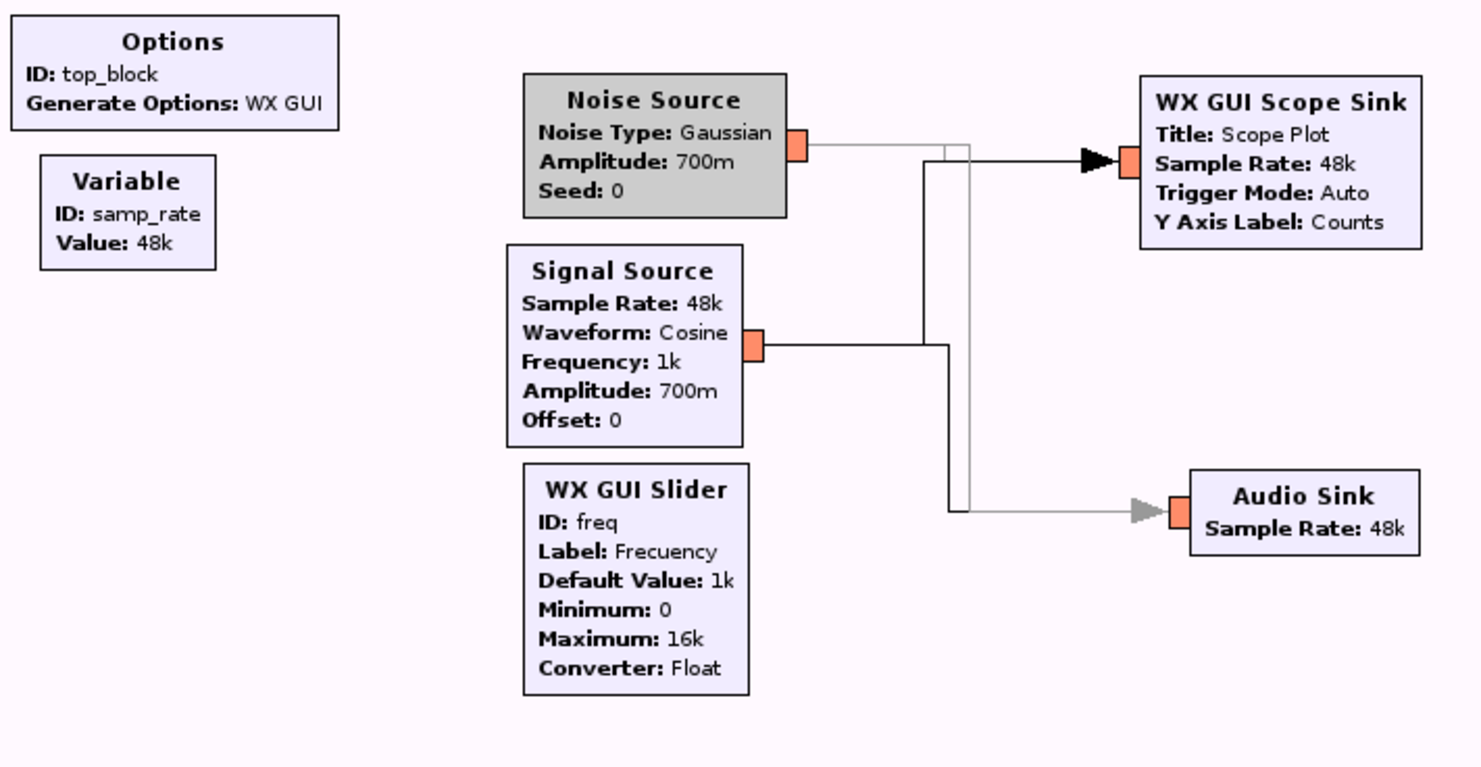
\includegraphics[width=\textwidth, height=0.4\textwidth]{lab3/pdf/lab30.pdf}
\end{figure}

\justifying
Emite un tono desde la tarjeta de sonido de la computadora.

\end{frame}


\begin{frame}[fragile]
\frametitle{Audio}
\justifying

\begin{figure}

\begin{center}
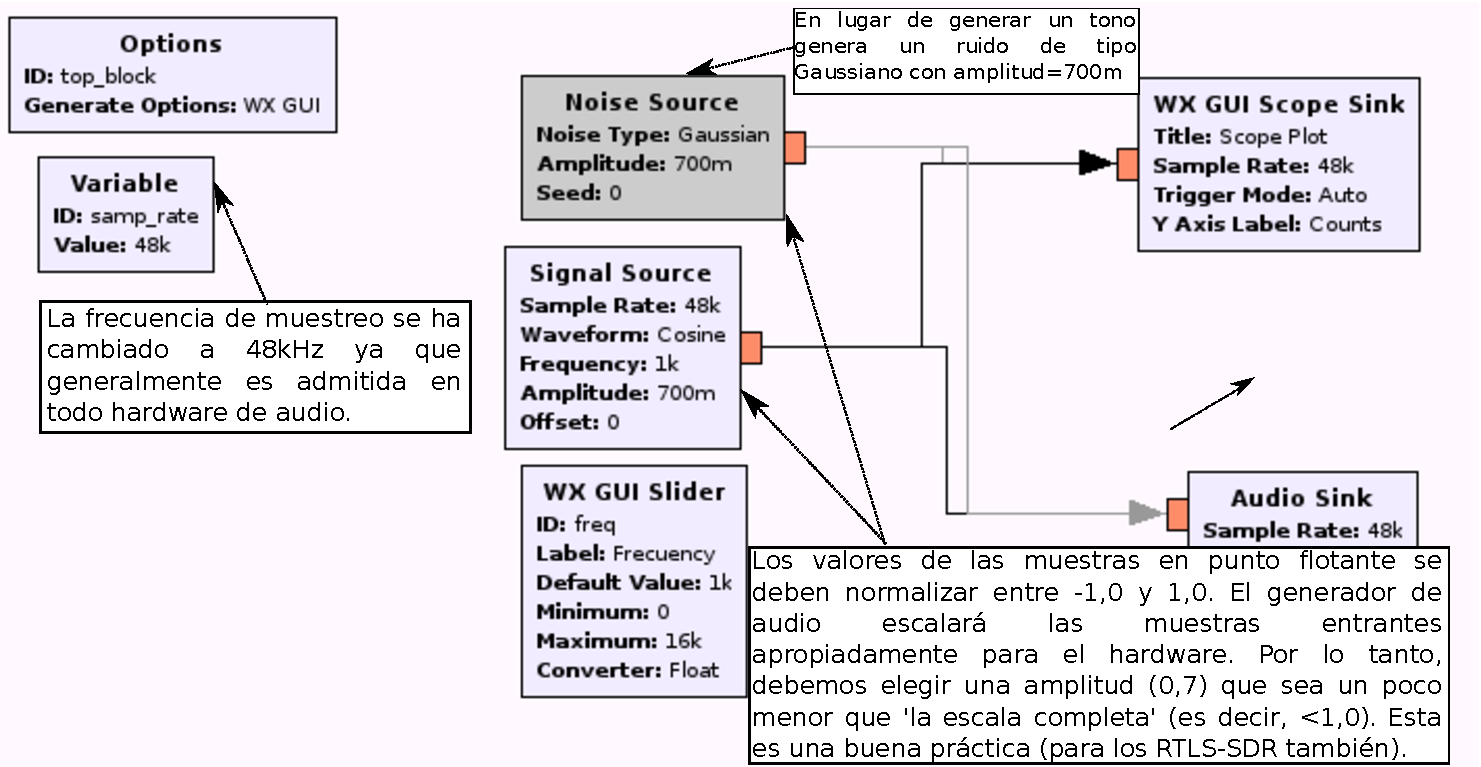
\includegraphics[width=\textwidth]{lab3/pdf/lab31.pdf}
\end{center}
\end{figure}
\end{frame}


\begin{frame}[fragile]
\frametitle{Audio}


\begin{figure}

\begin{center}
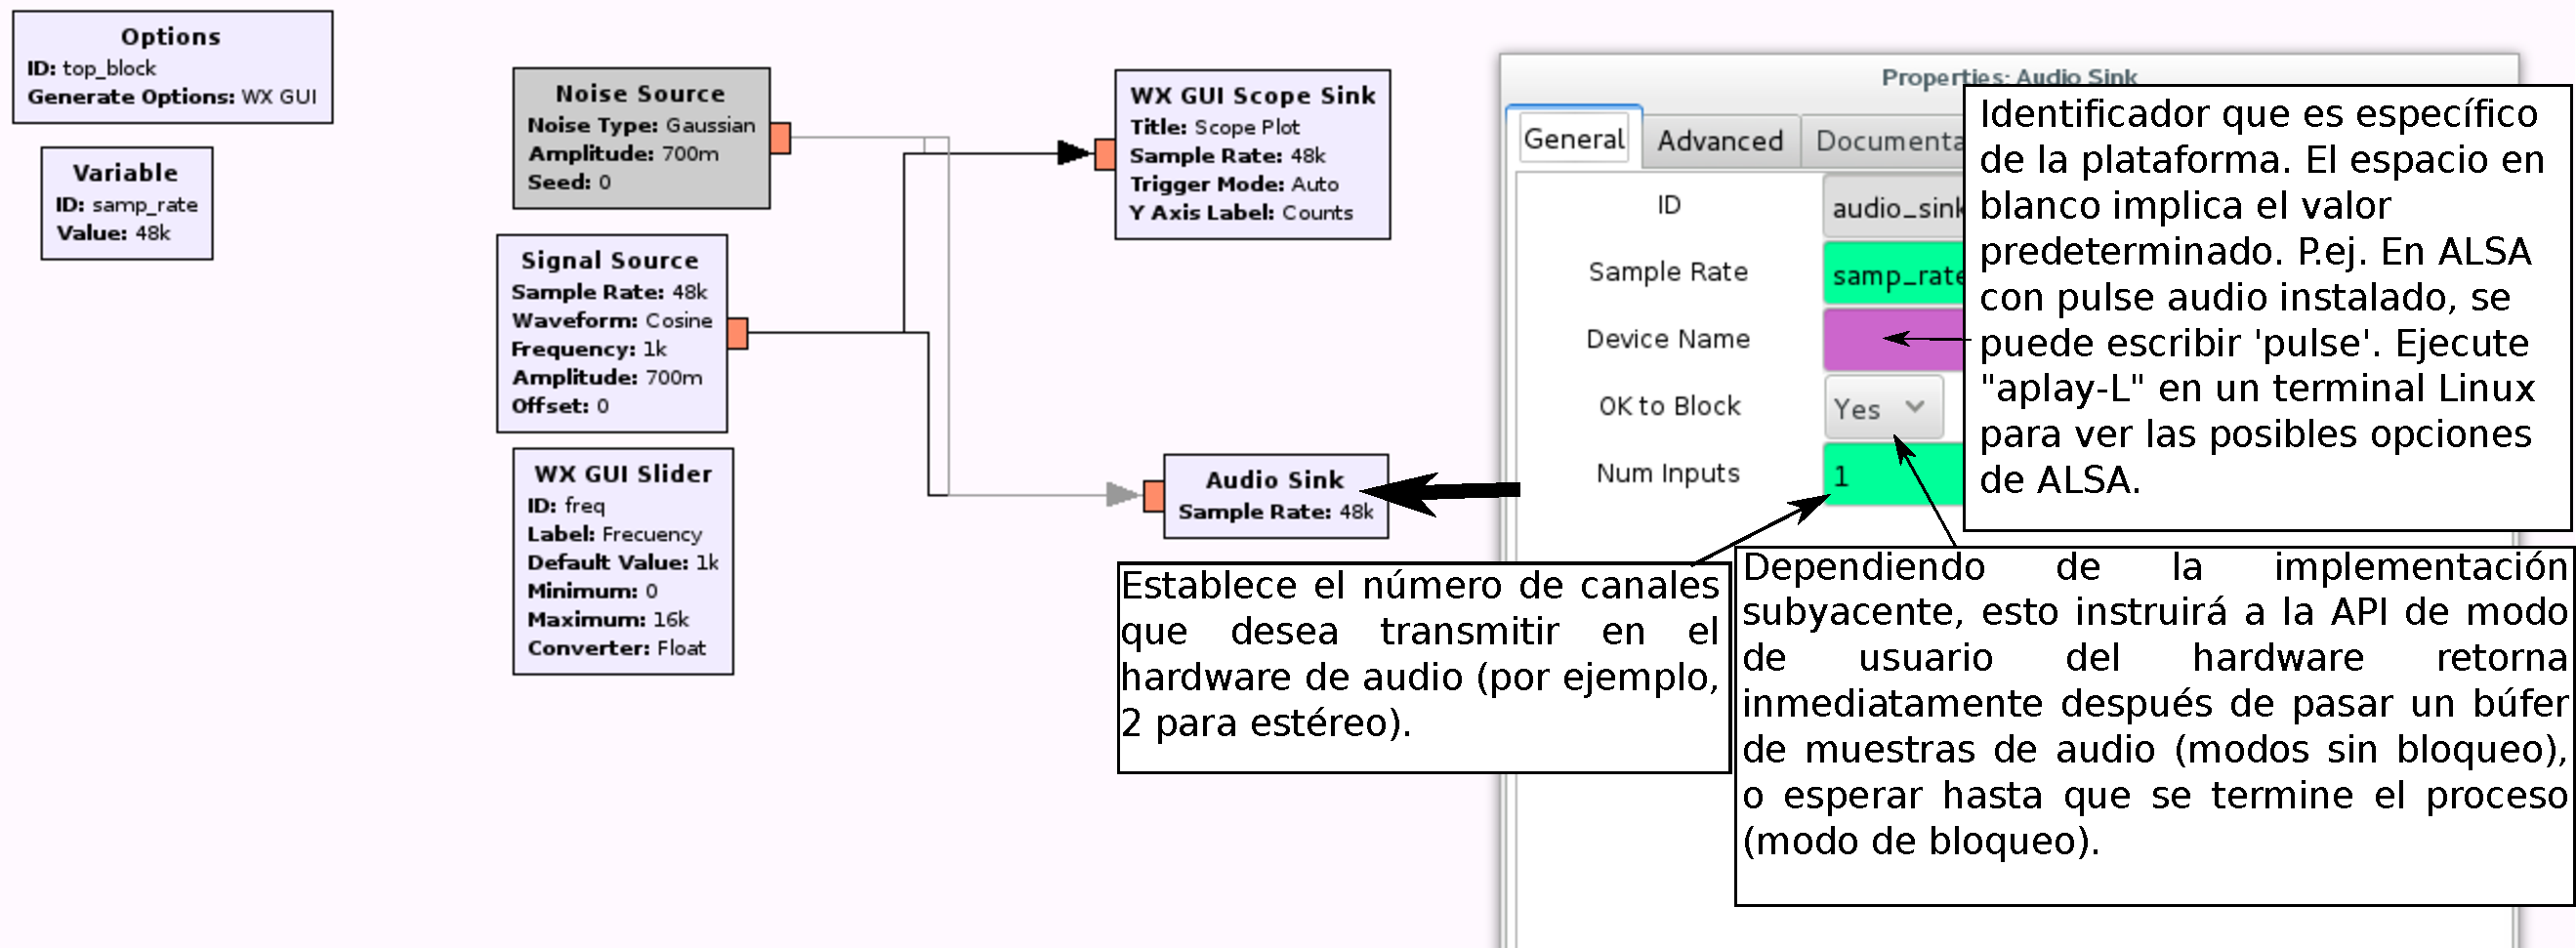
\includegraphics[width=0.9\paperwidth]{lab3/pdf/lab32.pdf}
\end{center}

\end{figure}
\end{frame}


\begin{frame}
\frametitle{Audio\index{OK to Block}}
\begin{itemize}
    \item El modo de bloqueo (‘OK to Block’) aplicará previamente un
    controlador regulado para que el Audio Sink opere eficazmente
    al escuchar el sonido, además es el único dispositivo del
    hardware en el diagrama de bloques capaz de emitir audio.
    \item Esto puede ser problemático si la fuente del diagrama de flujo
    es, por ejemplo, un RTL-SDR. La fuente es también un
    hardware que tiene su propio reloj interno y será regulado a la
    tasa de producción de las muestras, mientras que el Audio
    Sink regula el uso con su propio reloj no sincronizado. Esto se
    llama el problema de “dos relojes".
\end{itemize}
\end{frame}

\begin{frame}
\frametitle{Audio}
\begin{itemize}
    \item Para solucionar este problema de dos relojes, se coloca un
    regulador de audio en modo sin bloqueo (no dar click ‘Botón
    de Bloqueo’) de tal forma que nunca interrumpa el diagrama
    de bloque (es decir, no aplicar el regulador controlado). Esto
    usará muestras de forma normal, pero si hay un exceso (por
    ejemplo, el RTL-SDR está produciendo muestras un poco más
    rápido de lo que el Audio Sink puede usar), se caerán las
    muestras (podría causar fallas de audio).

    \item Esto no soluciona el caso en el que las muestras se producen
    más lentamente que la tasa de uso del Audio Sink (esto
    producirá una una ejecución lenta : el audio sonará agitado y
    se imprimirá ‘aU’ en la ventana de registro).

\end{itemize}
\end{frame}


\begin{frame}[fragile]
\frametitle{Audio}
\justifying

\begin{figure}

\begin{center}
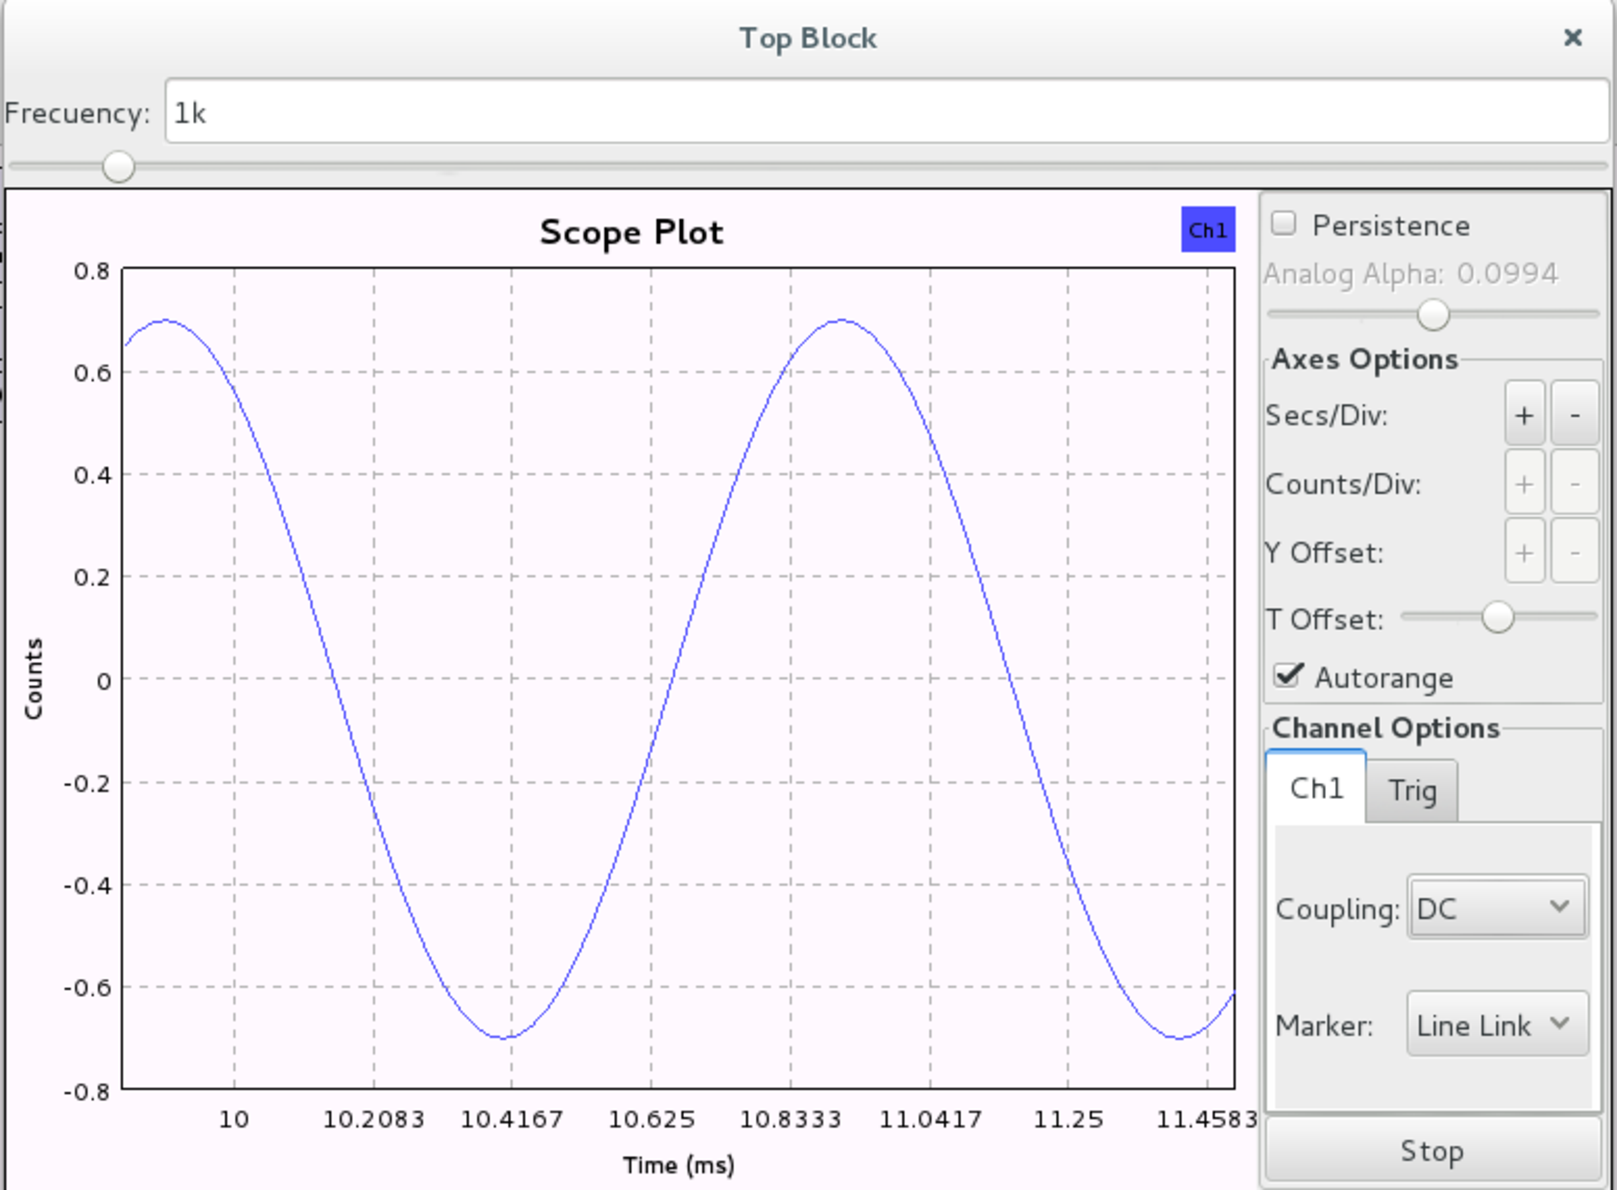
\includegraphics[scale=0.25]{lab3/pdf/lab33.pdf}

\end{center}

\end{figure}

\justifying
La misma onda seno de antes, pero ahora la escuchamos emitida
por los parlantes del computador.

\end{frame}

\begin{frame}[fragile]
\frametitle{Audio}
\justifying

\begin{figure}

\begin{center}
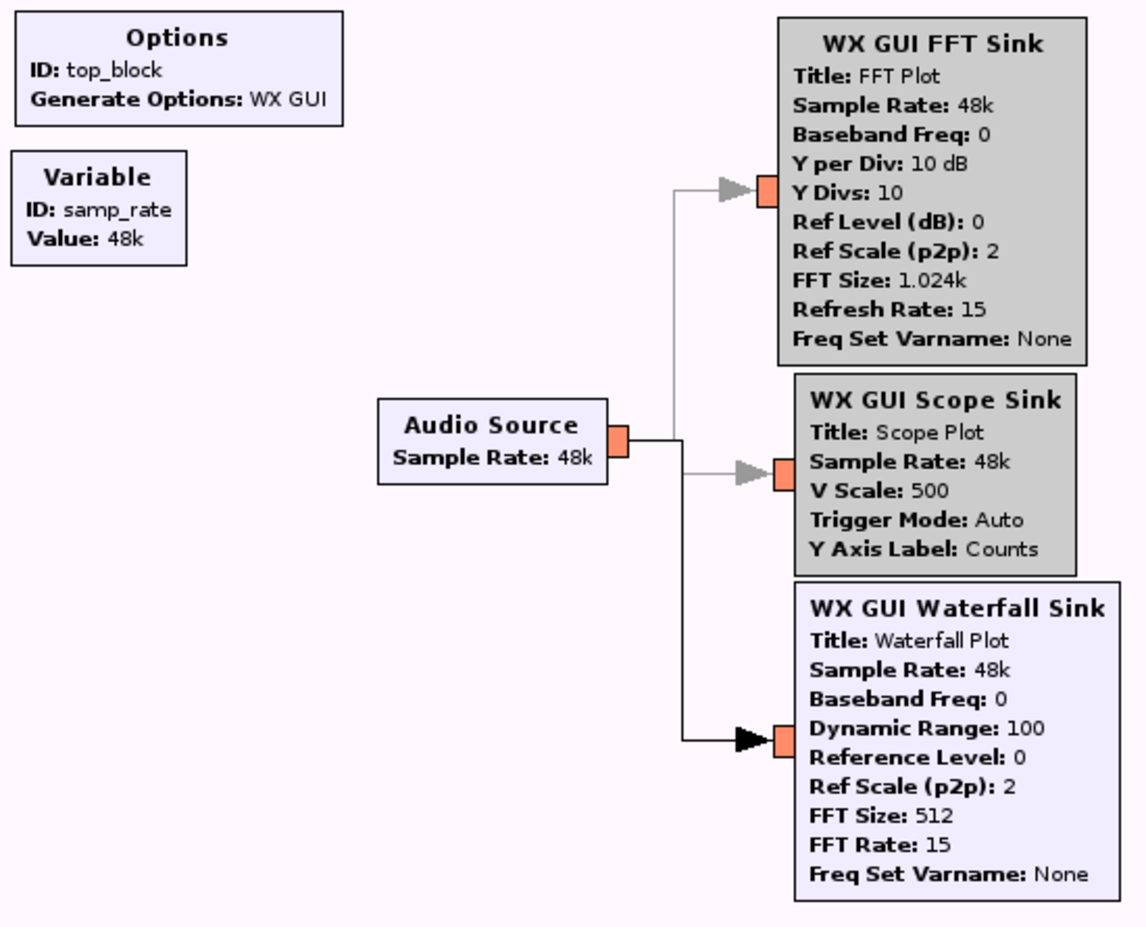
\includegraphics[scale=0.3]{lab3/pdf/lab34.pdf}

\end{center}

\end{figure}

\justifying
Visualiza el audio muestreado por la tarjeta de sonido en un FFT
que se desplaza en el tiempo mediante el diagrama de (cascada /
espectrograma).

\end{frame}

\begin{frame}[fragile]
\frametitle{Audio}
\justifying

\begin{figure}

\begin{center}
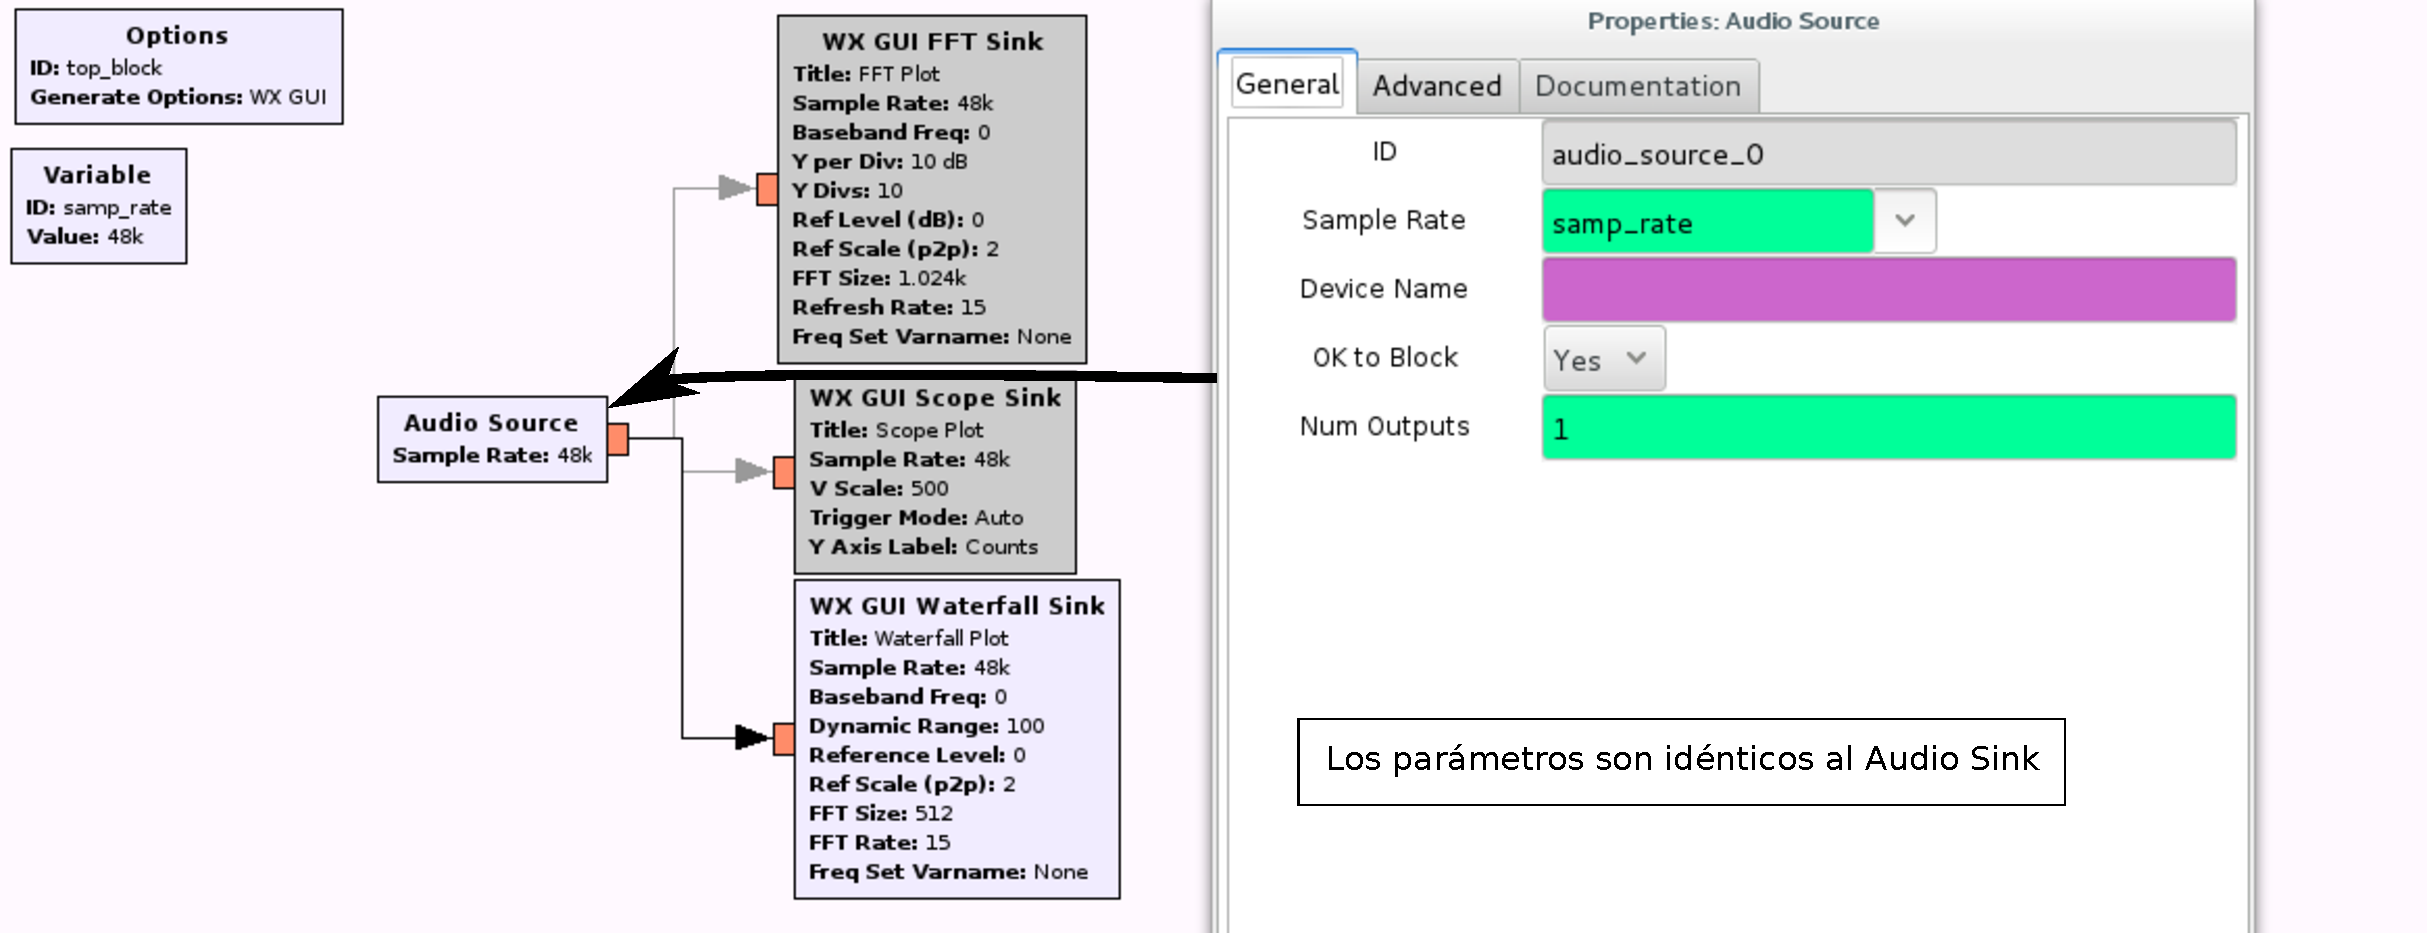
\includegraphics[width=\paperwidth,height=0.55\paperheight]{lab3/pdf/lab35.pdf}
\end{center}

\end{figure}

\end{frame}

\begin{frame}[fragile]
\frametitle{Audio}
\justifying

\begin{figure}

\begin{center}
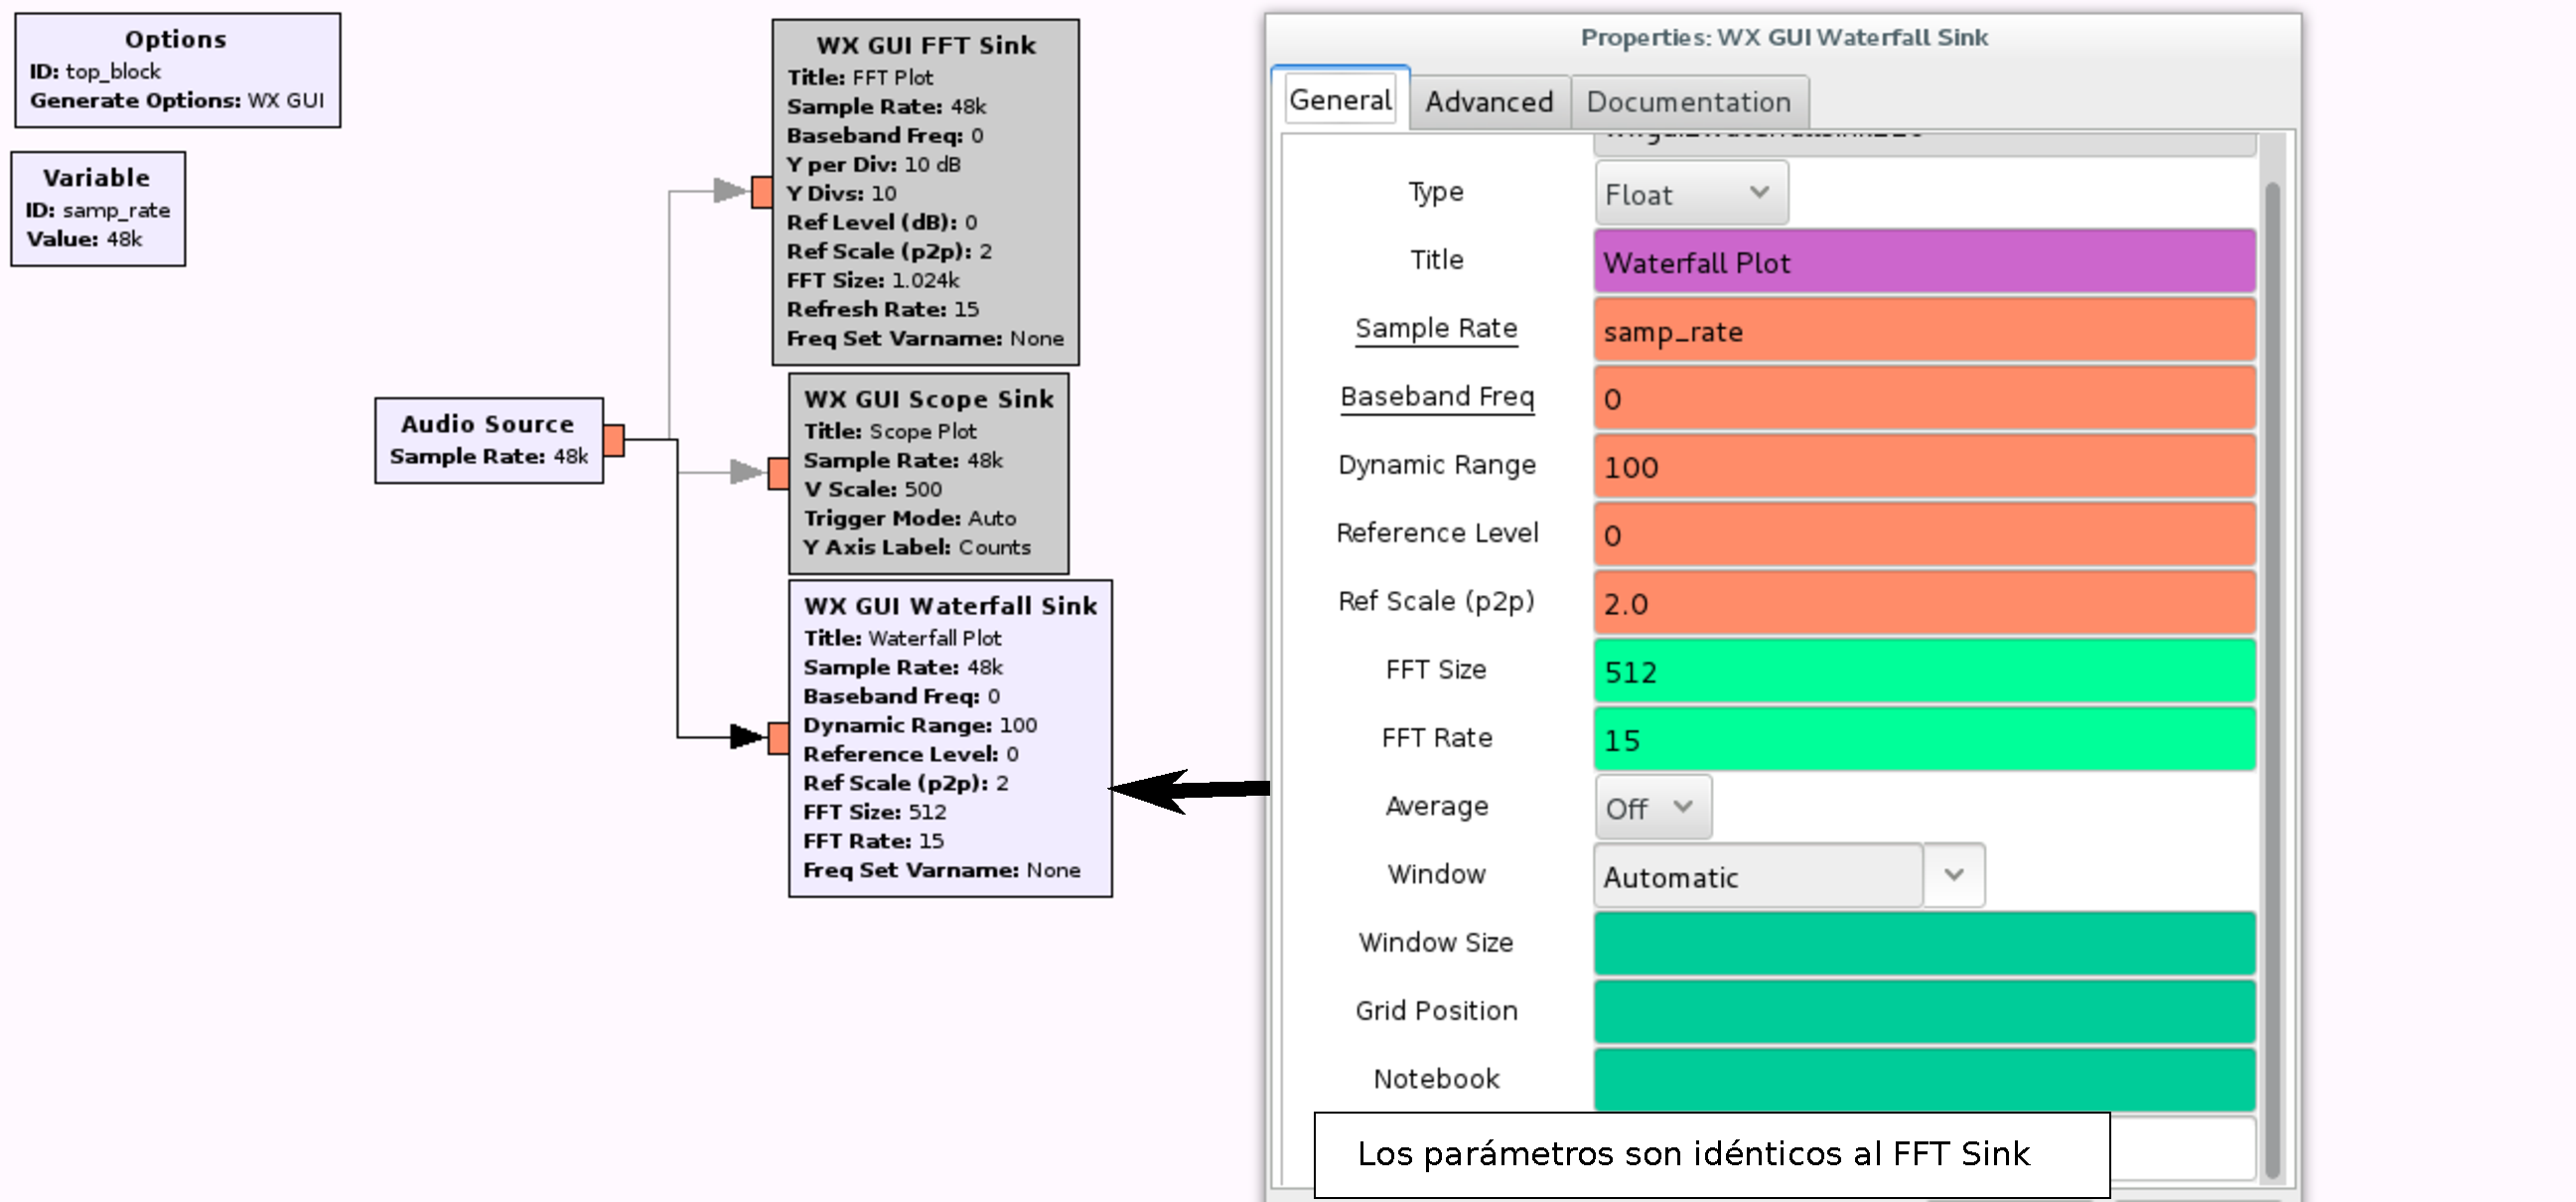
\includegraphics[width=\textwidth]{lab3/pdf/lab36.pdf}
\end{center}

\end{figure}

\end{frame}

\begin{frame}[fragile]
\frametitle{Audio}
\justifying

\begin{figure}

\begin{center}
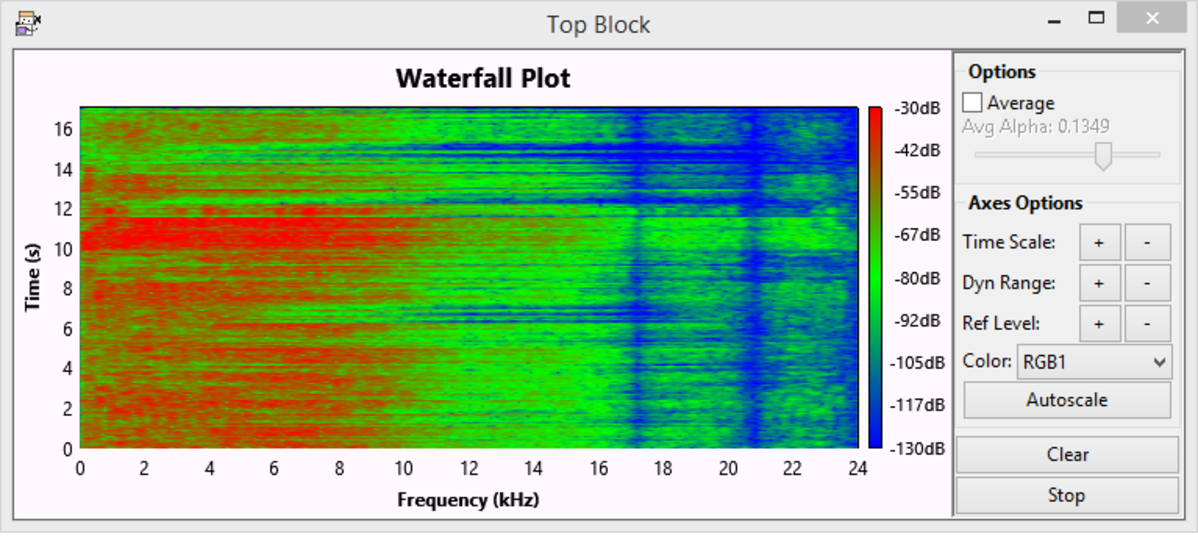
\includegraphics[width=\textwidth]{lab3/pdf/lab37.pdf}

\end{center}

\end{figure}

\justifying
Ejecutando el programa generador de onda senoidal al mismo
tiempo, y cambiando la frecuencia. Se trata de una prueba
aproximada de “loopback" en la que el micrófono de la
computadora escucha sus altavoces.


\end{frame}

\begin{frame}[fragile]
\frametitle{Audio}
\justifying

\begin{figure}

\begin{center}
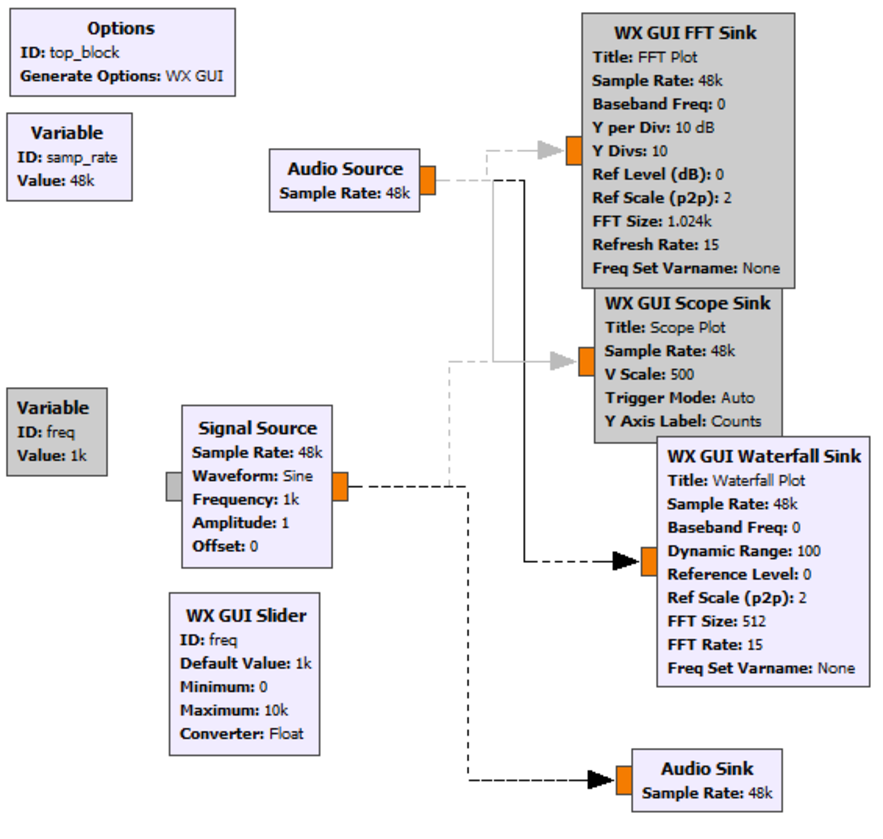
\includegraphics[scale=0.35]{lab3/pdf/lab38.pdf}

\end{center}

\end{figure}

\justifying
Se añade un bloque de prueba por medio de un generador de
señales y un variador deslizante lo cual se escucha el tono variado
en el Audio Sink y poder ver la variación de la frecuencia en el
diagrama de cascada.

\end{frame}

\begin{frame}[fragile]
\frametitle{Audio}
\justifying

\begin{figure}

\begin{center}
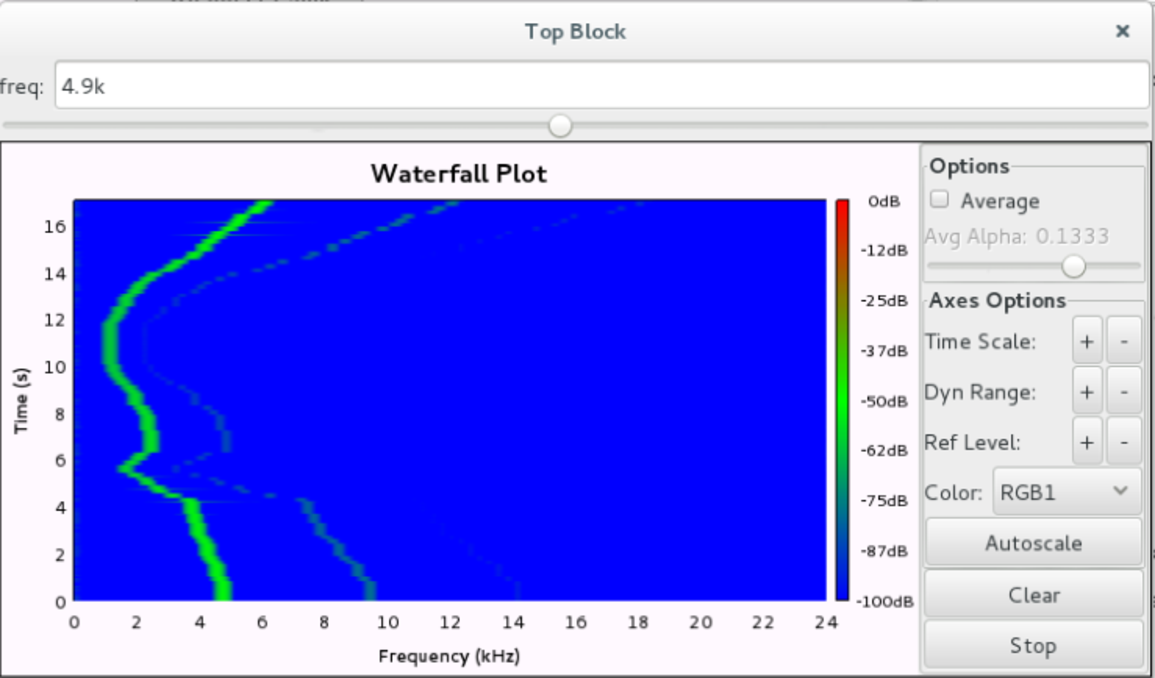
\includegraphics[scale=0.4]{lab3/pdf/lab39.pdf}

\end{center}

\end{figure}

\justifying
Ejecutando el programa generador de onda senoidal se muestra la
variación de frecuencia sin “loopback" del las entradas
micrófono-altavoces.

\end{frame}

\begin{frame}[fragile]
\frametitle{Audio}
\justifying

\begin{figure}

\begin{center}
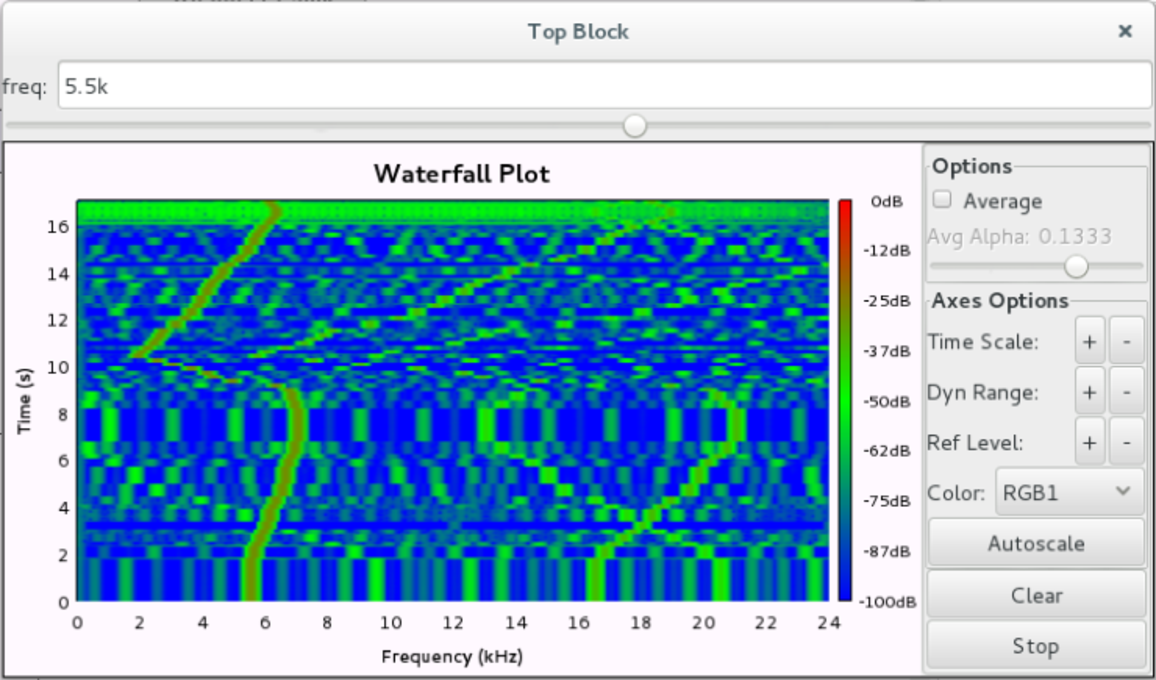
\includegraphics[scale=0.5]{lab3/pdf/lab310.pdf}

\end{center}

\end{figure}

\justifying
Con la retroalimentación del las entradas micrófono-altavoces.

\end{frame}